\documentclass[tikz,border=10pt]{standalone}
\usepackage{amsmath,amssymb}
\usepackage{tikz}
\usetikzlibrary{arrows,automata,backgrounds,calendar,chains,decorations,decorations.pathreplacing,decorations.text,fit,matrix,mindmap,patterns,petri,plotmarks,positioning,shadows,shapes,shapes.callouts,shapes.geometric,shapes.misc,spy,trees,calc,intersections,tikzmark,arrows.meta}
\usepackage{xcolor}
\usepackage{pgfplots}
\pgfplotsset{compat=1.16}

% Common math macros from the book
\def\x{\mathbf{x}}
\def\y{\mathbf{y}}
\def\z{\mathbf{z}}
\def\A{\mathbf{A}}
\def\b{\mathbf{b}}
\def\c{\mathbf{c}}
\def\w{\mathbf{w}}
\def\v{\mathbf{v}}
\def\u{\mathbf{u}}
\def\e{\mathbf{e}}
\def\zero{\mathbf{0}}
\def\R{\mathbb{R}}
\def\N{\mathbb{N}}
\def\Z{\mathbb{Z}}
\def\Q{\mathbb{Q}}
\def\st{\text{s.t.}}
\def\vect#1{\mathbf{#1}}
\def\xLP{x^{\mathrm{LP}}}
\def\zLP{z^{\mathrm{LP}}}
\def\xIP{x^{\mathrm{IP}}}

% Common node styles from the book
\tikzset{
    main/.style={circle, draw, fill=gray!20, minimum size=1cm, font=\normalsize},
    dot/.style={circle,fill=blue,minimum size=3pt,inner sep=0pt, outer sep=-1pt},
    vertex/.style={circle,fill=black!25,minimum size=20pt,inner sep=0pt},
    edge/.style={draw,-,thick},
    directed edge/.style={draw,->,>=latex,thick},
}

% Additional macros for 3D/coordinate systems
\newcommand{\xhat}{\hat{\x}}
\newcommand{\yhat}{\hat{\y}}
\newcommand{\zhat}{\hat{\z}}
\newcommand{\ihat}{\hat{\imath}}
\newcommand{\jhat}{\hat{\jmath}}
\newcommand{\khat}{\hat{k}}

\begin{document}
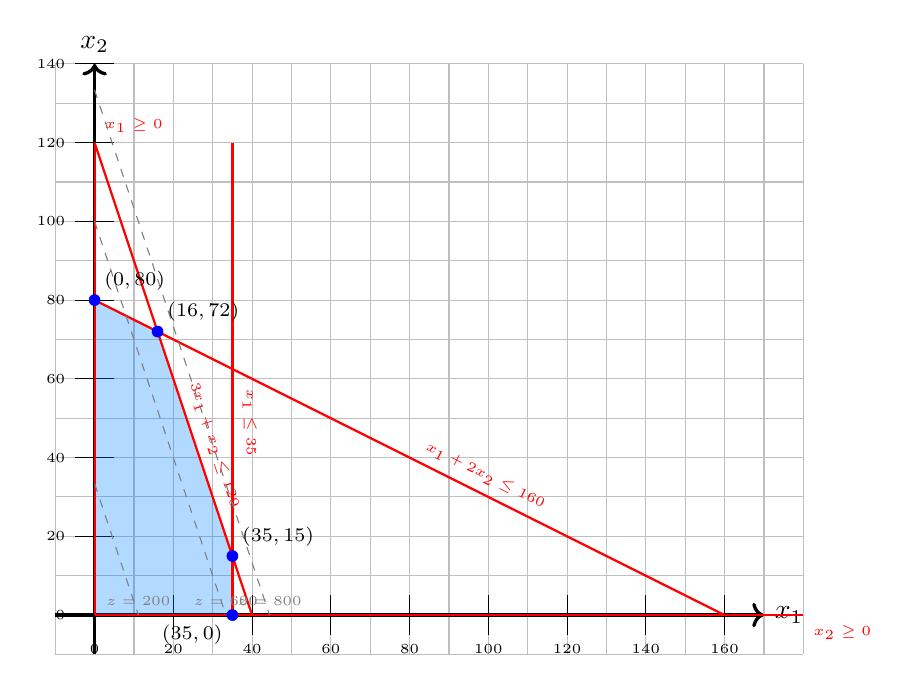
\begin{tikzpicture}[scale=0.05]
    % Grid and axes
    \draw[gray!50, thin, step=10] (-10,-10) grid (180,140);
    \draw[very thick,->] (-10,0) -- (170,0) node[right] {$x_1$};
    \draw[very thick,->] (0,-10) -- (0,140) node[above] {$x_2$};

    % Axis labels
    \foreach \x in {0,20,...,160} \draw (\x,5) -- (\x,-5) node[below] {\tiny\x};
    \foreach \y in {0,20,...,140} \draw (5,\y) -- (-5,\y) node[left] {\tiny\y};

    % Feasible region vertices
    \fill[blue!50!cyan,opacity=0.3] 
        (0,0) -- (0,80) -- (16,72) -- (35,15) -- (35,0) -- cycle;

    % Constraint lines

    \draw[red,thick] (0,120/1) --  node[above right, sloped] {\tiny $3x_1 + x_2 \leq 120$}(120/3,0);
    \draw[red,thick] (0,160/2) --  node[above right, sloped] {\tiny $x_1 + 2x_2 \leq 160$}(160,0);
    \draw[red,thick] (35,120) --  node[above right, sloped] {\tiny $x_1 \leq 35$}(35,0);
    \draw[red,thick] (0,0) -- (180,0) node[below right] {\tiny $x_2 \geq 0$};
    \draw[red,thick] (0,0) -- (0,120) node[above right] {\tiny $x_1 \geq 0$};

    % Objective function contours
    \draw[dashed,gray] (0,600/6) -- (600/18,0) node[above, sloped ] {\tiny $z = 600$};
    \draw[dashed,gray] (0,800/6) -- (800/18,0) node[above ] {\tiny $z = 800$};
    \draw[dashed,gray] (0,200/6) -- (200/18,0) node[above, sloped ] {\tiny $z = 200$};

    % Labels for vertices
    \node[blue] at (0,80) [circle,fill,inner sep=1.5pt]{};
    \node[blue] at (16,72) [circle,fill,inner sep=1.5pt]{};
    \node[blue] at (35,15) [circle,fill,inner sep=1.5pt]{};
    \node[blue] at (35,0) [circle,fill,inner sep=1.5pt]{};

    % Vertex coordinates
    \node[black,anchor=south west] at (0,80) {\scriptsize $(0,80)$};
    \node[black,anchor=south west] at (16,72) {\scriptsize $(16,72)$};
    \node[black,anchor=south west] at (35,15) {\scriptsize $(35,15)$};
    \node[black,anchor=north east] at (35,0) {\scriptsize $(35,0)$};

    % Objective function label
    %\node[gray] at (30,140) {\tiny $7x_1 + 6x_2 = z$};
\end{tikzpicture}
\end{document}
